\section{Methodology}
\label{sec:Modelling Approach}

The following sections describe the model architecture and training strategy, as well as the reasoning behind them. 

\subsection{Convolutional Autoencoder}
\label{subsec:Model Architecture}
We used convolutional autoencoder(CAE) as our first model. This type of network is composed of two parts, an encoder in charge of compressing the input into a smaller latent representation, and a decoder in charge of reconstructing the original input. When trained with normal samples only, the network learns to perform the reconstruction process just for this type of input; thus, it will fail when reconstructing anomaly samples, generating a higher reconstruction error that exposes the presence of an anomaly.

However, as data now have a grid-like representation, convolutional layers are implemented within the network to exploit their capabilities to capture localized patterns as often anomalies are exposed in specific regions from the frequency domain. Additionally, the convolutional layer parameter sharing feature helps them to detect patterns anywhere in the spectrograms, which makes use of the stationary condition of audio signals and their anomalies. When combined to create deep architectures they can learn composite representations from different levels, from short frequency peaks in a low level scale to engine sounds in a much higher scale.

\textbf{Specifications}

The implemented model uses a symmetric architecture consisting of an encoder and a decoder, connected through a fully connected bottleneck layer in the latent space. The encoder comprises three convolutional layers, each with a kernel size of 3, followed by ReLU activation functions and max-pooling operations for spatial downsampling. The decoder mirrors this structure using transposed convolutional layers to up-sample from the latent representation, again followed by ReLU activations. The model is defined by the pseudocode below:

% \begin{mdframed}[backgroundcolor=gray!20]
% \begin{minted}[breaklines]{python}
% latent_dim=256

% # Encoder
% self.enc = nn.Sequential(
%     nn.Conv2d(1, 16, kernel_size=3, padding=1), nn.ReLU(), 
%     nn.MaxPool2d(2),                   
%     nn.Conv2d(16, 32, kernel_size=3, padding=1), nn.ReLU(),
%     nn.MaxPool2d(2),                   
%     nn.Conv2d(32, 64, kernel_size=3, padding=1), nn.ReLU(),
%     nn.MaxPool2d(2),)

% # Fully connected layers
% self.enc_fc = nn.Sequential(
%     nn.Flatten(), nn.Linear(64 * 8 * 39, latent_dim))

% self.dec_fc = nn.Sequential(
%     nn.Linear(latent_dim, 64 * 8 * 39), nn.Unflatten(1, (64, 8, 39)))

% # Decoder
% self.dec = nn.Sequential(
%     nn.ConvTranspose2d(64, 32, kernel_size=4, stride=2, padding=1), nn.ReLU(),
%     nn.ConvTranspose2d(32, 16, kernel_size=4, stride=2, padding=1), nn.ReLU(),
%     nn.ConvTranspose2d(16, 1, kernel_size=4, stride=2, padding=1),)

% # Final 1x1 conv to pad to 313
% self.pad_to_313 = nn.ConstantPad2d((0, 1, 0, 0), 0)
% \end{minted}
% \end{mdframed}

\begin{algorithm}[H]
\caption{Convolutional Autoencoder with Constant Padding}
\KwData{Log--Mel spectrogram $\mathbf X \in \mathbb{R}^{1 \times 64 \times 313}$}
\KwResult{Reconstructed spectrogram $\hat{\mathbf X}$}

% -------------------------------------------------
% Hyper-parameter
\SetKwComment{tcp}{//}{}
\SetKwProg{Fn}{Function}{}{}
\DontPrintSemicolon

\tcp*[l]{\textbf{Hyper-parameter}}
$\textit{latent\_dim} \leftarrow 256$\;

\BlankLine
% -------------------------------------------------
% Encoder
\tcp*[l]{\textbf{Encoder}}
$\mathbf H \leftarrow \mathrm{Conv2D}(1,16,3,1)\!\circ\!\mathrm{ReLU}\!\circ\!\mathrm{MaxPool2D}(2)(\mathbf X)$\;
$\mathbf H \leftarrow \mathrm{Conv2D}(16,32,3,1)\!\circ\!\mathrm{ReLU}\!\circ\!\mathrm{MaxPool2D}(2)(\mathbf H)$\;
$\mathbf H \leftarrow \mathrm{Conv2D}(32,64,3,1)\!\circ\!\mathrm{ReLU}\!\circ\!\mathrm{MaxPool2D}(2)(\mathbf H)$\tcp*{output size $64\times8\times39$}

\BlankLine
% -------------------------------------------------
% Bottleneck
\tcp*[l]{\textbf{Fully-connected bottleneck}}
$\mathbf z \leftarrow \mathrm{Linear}(64\!\cdot\!8\!\cdot\!39,\ \textit{latent\_dim})\!\circ\!\mathrm{Flatten}(\mathbf H)$\;

\BlankLine
% -------------------------------------------------
% Inverse bottleneck
\tcp*[l]{\textbf{Decoder (inverse FC)}}
$\mathbf H' \leftarrow \mathrm{Unflatten}\!\circ\!\mathrm{Linear}(\textit{latent\_dim},64\!\cdot\!8\!\cdot\!39)(\mathbf z)$\;

\BlankLine
% -------------------------------------------------
% Decoder
\tcp*[l]{\textbf{Decoder (deconvolutions)}}
$\mathbf H' \leftarrow \mathrm{ConvTr2D}(64,32,4,2,1)\!\circ\!\mathrm{ReLU}(\mathbf H')$\;
$\mathbf H' \leftarrow \mathrm{ConvTr2D}(32,16,4,2,1)\!\circ\!\mathrm{ReLU}(\mathbf H')$\;
$\hat{\mathbf X} \leftarrow \mathrm{ConvTr2D}(16,1,4,2,1)(\mathbf H')$\;

\BlankLine
% -------------------------------------------------
% Padding
\tcp*[l]{\textbf{Final padding to width $313$}}
$\hat{\mathbf X} \leftarrow \mathrm{ConstantPad2D}((0,1,0,0),\,0)(\hat{\mathbf X})$\;

\end{algorithm}

% The latent dimension was set to 256, as initial experiments showed that smaller latent sizes led to poor reconstruction performance on the validation set. This is likely because a latent space that is too small cannot effectively capture the underlying structure and variability of the input data.

The convolutional autoencoder (CAE) processes a log-Mel spectrogram input of size $64 \times 313$ (frequency $\times$ time). The encoder consists of three convolutional blocks with increasing filter widths ($32 \rightarrow 64 \rightarrow 128$), where each block is followed by batch normalisation and ReLU activation. Max-pooling layers progressively reduce the spatial resolution until a latent representation of dimension $2048$ is obtained.

The decoder mirrors the encoder architecture using transposed convolutions and terminates with a sigmoid activation layer that reconstructs the input resolution.

Training is performed using the mean squared error (MSE) loss and the Adam optimiser, with an initial learning rate of $1 \times 10^{-3}$, which is adjusted using the \texttt{ReduceLROnPlateau} scheduler. A dropout rate of $0.2$ is applied to regularise training, and early stopping is employed with a patience of 10 epochs to prevent overfitting. In practice, the model converges in approximately 45 epochs and contains around 1.2 million parameters, making it compact enough for deployment on edge GPUs.

\subsection{Support Vector Data Description}
For comparison, we implement \textit{Support Vector Data Description} (SVDD) with a radial basis function (RBF) kernel. Instead of using the full spectrogram as input, we feed a 128-dimensional summary vector that comprises the mean and variance of each Mel frequency band. The input vectors are standardised to have zero mean and unit variance. 

% ---------- Algorithm: SVDDNet Encoder ----------
\begin{algorithm}[H]
\caption{SVDDNet\,—\,Convolutional Encoder for Deep-SVDD}
\KwData{Mini-batch of log–Mel spectrograms $\mathbf X \in \mathbb R^{B\times1\times H\times W}$}
\KwResult{Embedding matrix $\mathbf Z \in \mathbb R^{B\times \textit{emb\_dim}}$}

\SetKwComment{tcp}{//}{}
\SetKwProg{Fn}{Function}{}{}        % ← inisialisasi macro \Fn
\DontPrintSemicolon

% -------------------------------------------------
\tcp*[l]{\textbf{Hyper-parameter}}
\textit{emb\_dim} $\leftarrow 128$\;

\vspace{0.3em}
% -------------------------------------------------
\tcp*[l]{\textbf{Constructor} (\_init\_)}
\textbf{define} $\mathrm{conv}$ as:\;
\Indp
$\mathrm{Conv2D}(1,16,3,\,\text{pad}=1)\!\rightarrow\!\mathrm{ReLU}\!\rightarrow\!\mathrm{MaxPool2D}(2)$\;
$\mathrm{Conv2D}(16,32,3,\,\text{pad}=1)\!\rightarrow\!\mathrm{ReLU}\!\rightarrow\!\mathrm{MaxPool2D}(2)$\;
$\mathrm{Flatten}$\;
\Indm

\BlankLine
% ---------- dynamic output shape ----------
\tcp{Compute the flattened dimension dynamically}
$\mathbf X_{\text{dummy}} \leftarrow$ one batch from \textit{train\_loader}\;
$\mathbf h \leftarrow \mathrm{conv}(\mathbf X_{\text{dummy}})$\;
$\textit{flat\_dim} \leftarrow \operatorname{dim}(\mathbf h,\,1)$\;

\BlankLine
\textbf{define} $\mathrm{fc} \leftarrow \mathrm{Linear}(\textit{flat\_dim},\,\textit{emb\_dim})$\;

\BlankLine
% -------------------------------------------------
\Fn{\textnormal{\textbf{forward}}($\mathbf X$)}{
    $\mathbf h \leftarrow \mathrm{conv}(\mathbf X)$\;
    $\mathbf Z \leftarrow \mathrm{fc}(\mathbf h)$\;
    \Return $\mathbf Z$\;
}

\end{algorithm}

Although SVDD is memory‑light and suitable for edge devices, its decision boundary is limited to global statistics and struggles with subtle, localised spectral modulations.

\subsection{Training Procedure}
\label{subsec:Training Procedure}

% The model was trained for 50 epochs, with performance monitored on the validation set after each epoch. Mean Squared Error (MSE) is used as loss function, as the objective is to accurately reconstruct the input. A lower MSE indicates a better reconstruction. After each epoch, the average MSE on the validation set was calculated, in order to track the models progression. 

% In addition, the model uses Adam optimization, which was chosen due to its efficiency in neural network architectures. The learning rate was set to 1e-3, which yielded the best convergence over the given epochs. \textcolor{red}{Will maybe add some grid search}

The study trains \textbf{two complementary one–class models}---a
\emph{convolutional auto-encoder} (CAE) and a \emph{Deep Support Vector
Data Description} network (Deep-SVDD)---exclusively on \textit{normal}
recordings from the \textit{dev\_train} split.  Both pipelines are implemented in
\textsc{PyTorch} with identical random seeds to ensure result reproducibility.

% ..................................................................

\paragraph{Convolutional Auto-Encoder (CAE).}
The CAE is trained for \textbf{50 epochs}, minimising the
mean-squared-error (MSE) between input and reconstruction.
A grid search over learning‐rate/batch‐size pairs
$\{1,3\}\!\times\!10^{-4, -3}\times\{16,32,64\}$
selects Adam with
$\alpha = 1\!\times\!10^{-3}$, $\beta_{1}=0.9$, $\beta_{2}=0.999$ and
batch size~32 as the most stable configuration; the same hyper-parameters
are used throughout.  
Early-stopping on a 10\,\% validation slice prevents over-fitting.

\vspace{0.4em}
\noindent

\textit{Qualitative check.}  

\begin{figure}[t]
  \centering
  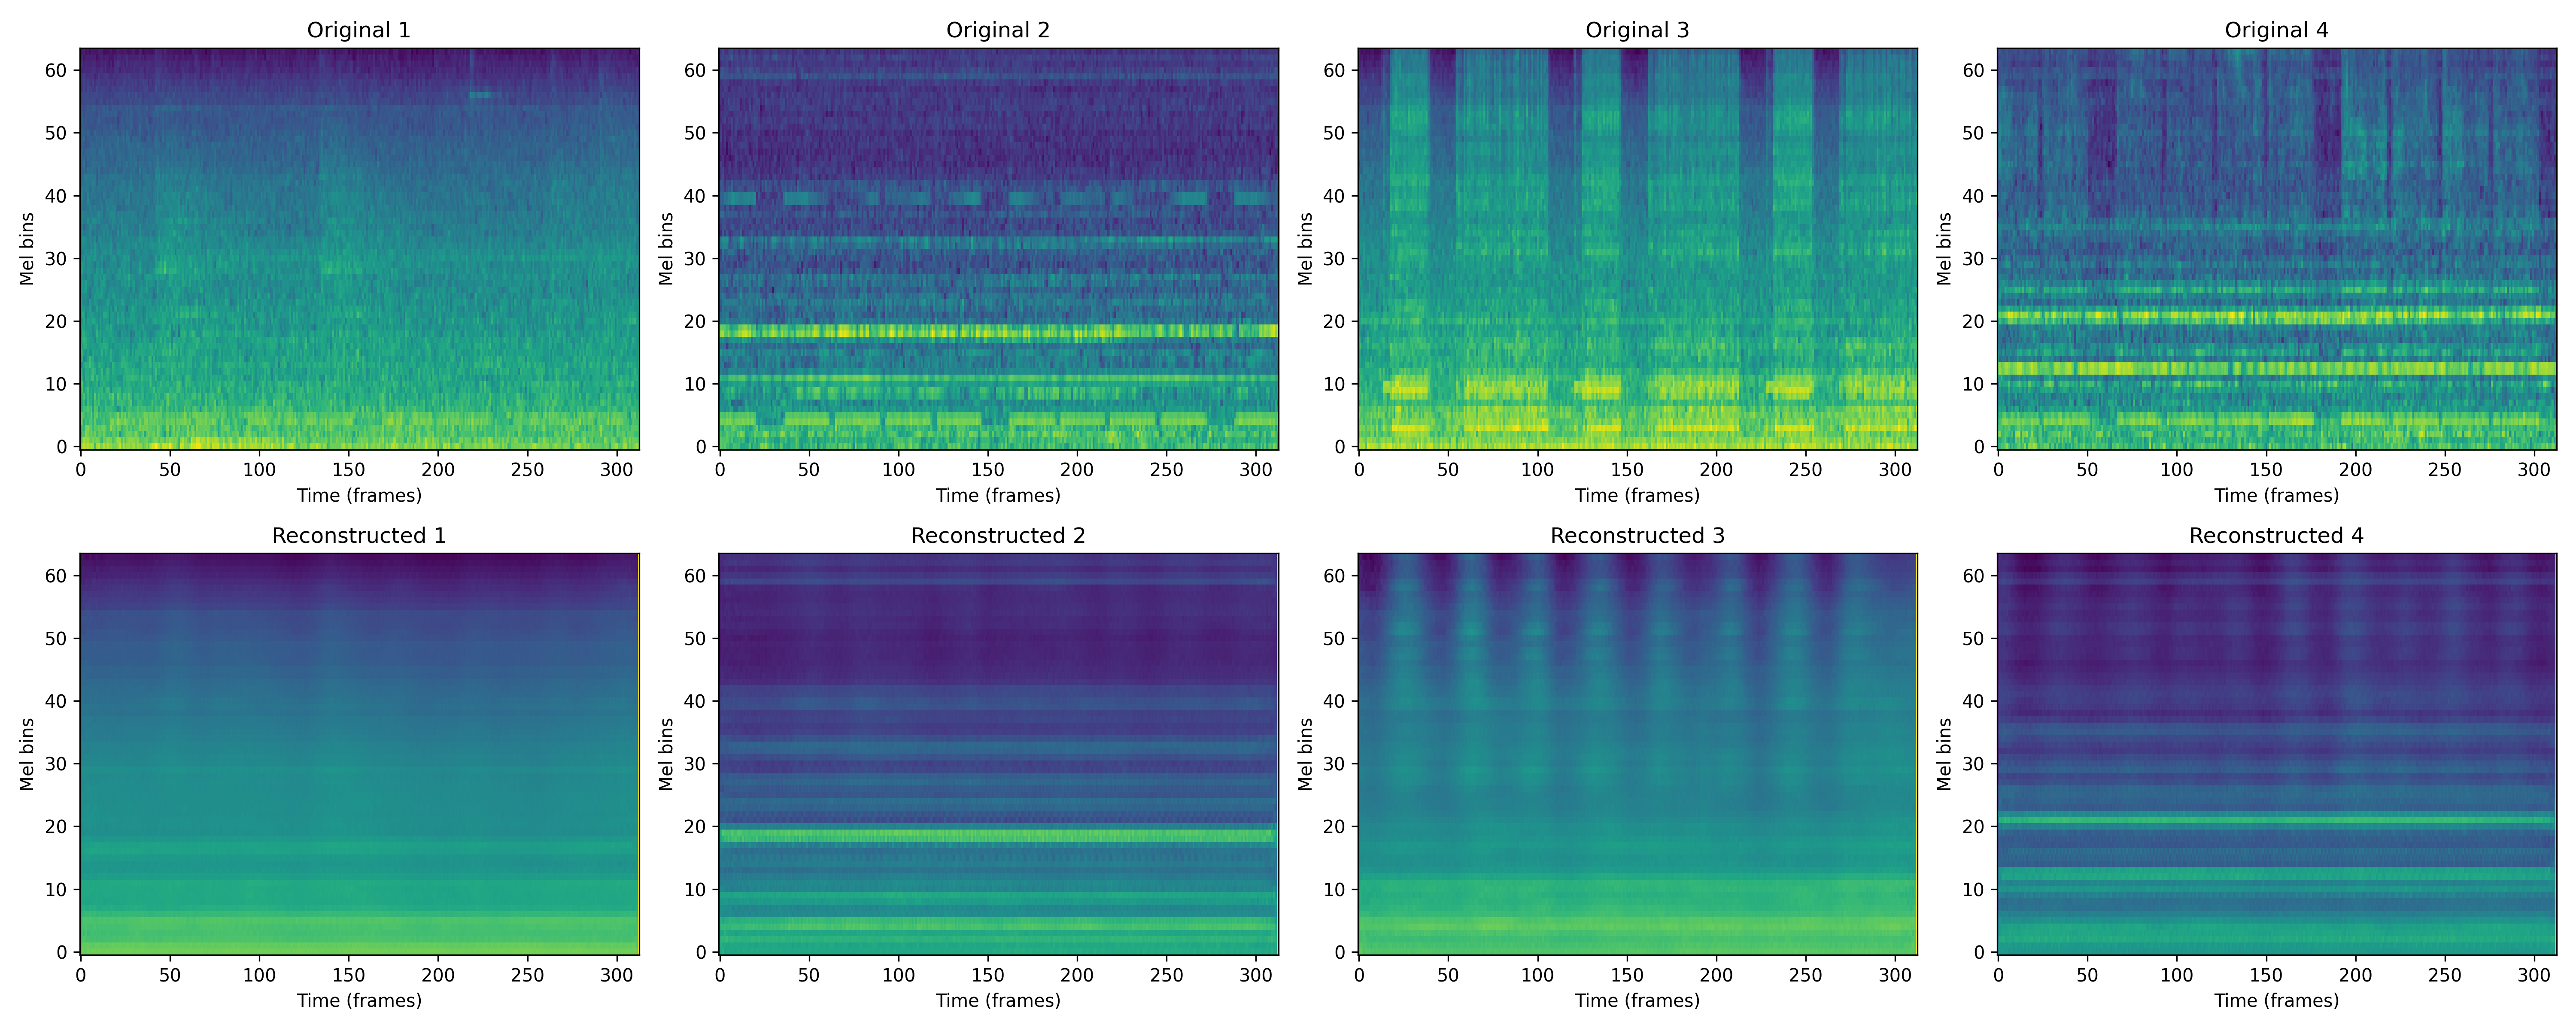
\includegraphics[width=\textwidth]{Figures/fig_reconstruction_examples_epoch24.png}
  \caption{Original (\emph{top}) versus reconstructed (\emph{bottom})
           log-Mel spectrograms produced by the CAE at epoch~24.
           Columns~1–2 are normal samples; Columns~3–4 are anomalous
           samples.  Normal inputs are faithfully reconstructed, whereas
           anomalies display spectral distortion, confirming the use of
           reconstruction error as an anomaly score.}
  \label{fig:recon_examples}
\end{figure}

Figure~\ref{fig:recon_examples} contrasts original and reconstructed
log-Mel spectrograms at epoch~24.  Normal inputs are reproduced almost
perfectly, whereas anomalous inputs incur visible spectral artefacts,
indicating higher reconstruction errors that are later exploited at
inference time.

% ..................................................................

\paragraph{Deep-SVDD.}
For the Deep-SVDD branch we adopt the soft-boundary objective.  
The feature extractor consists of three $3{\times}3$ convolutional
blocks (16-32-64 filters) followed by a fully connected layer that maps
to a \textbf{128-dimensional} embedding; all layers use ReLU activations
and $2{\times}2$ max-pooling.  

Training proceeds for \textbf{10 epochs} with Adam
($\alpha = 1\!\times\!10^{-4}$, batch size~64).
At the first forward pass, the hypersphere centre $c\!\in\!\mathbb{R}^{128}$
is initialised as the mini-batch mean; thereafter it is updated with a
moving average  
$c \leftarrow 0.9\,c + 0.1\,\bar{e}^{(t)}$,  
where $\bar{e}^{(t)}$ denotes the batch mean embedding at iteration~$t$.
The loss minimises the squared Euclidean distance
$\lVert e_i - c\rVert^{2}$ for each sample~$e_i$, thus compacting normal
embeddings around~$c$.  
A shorter training horizon suffices because the objective converges
quickly once the centre stabilises, and longer runs risk
hypersphere collapse.

\vspace{0.4em}
\noindent